%UCC-1: Utilizzo artefatto

\begin{figure}
\centering
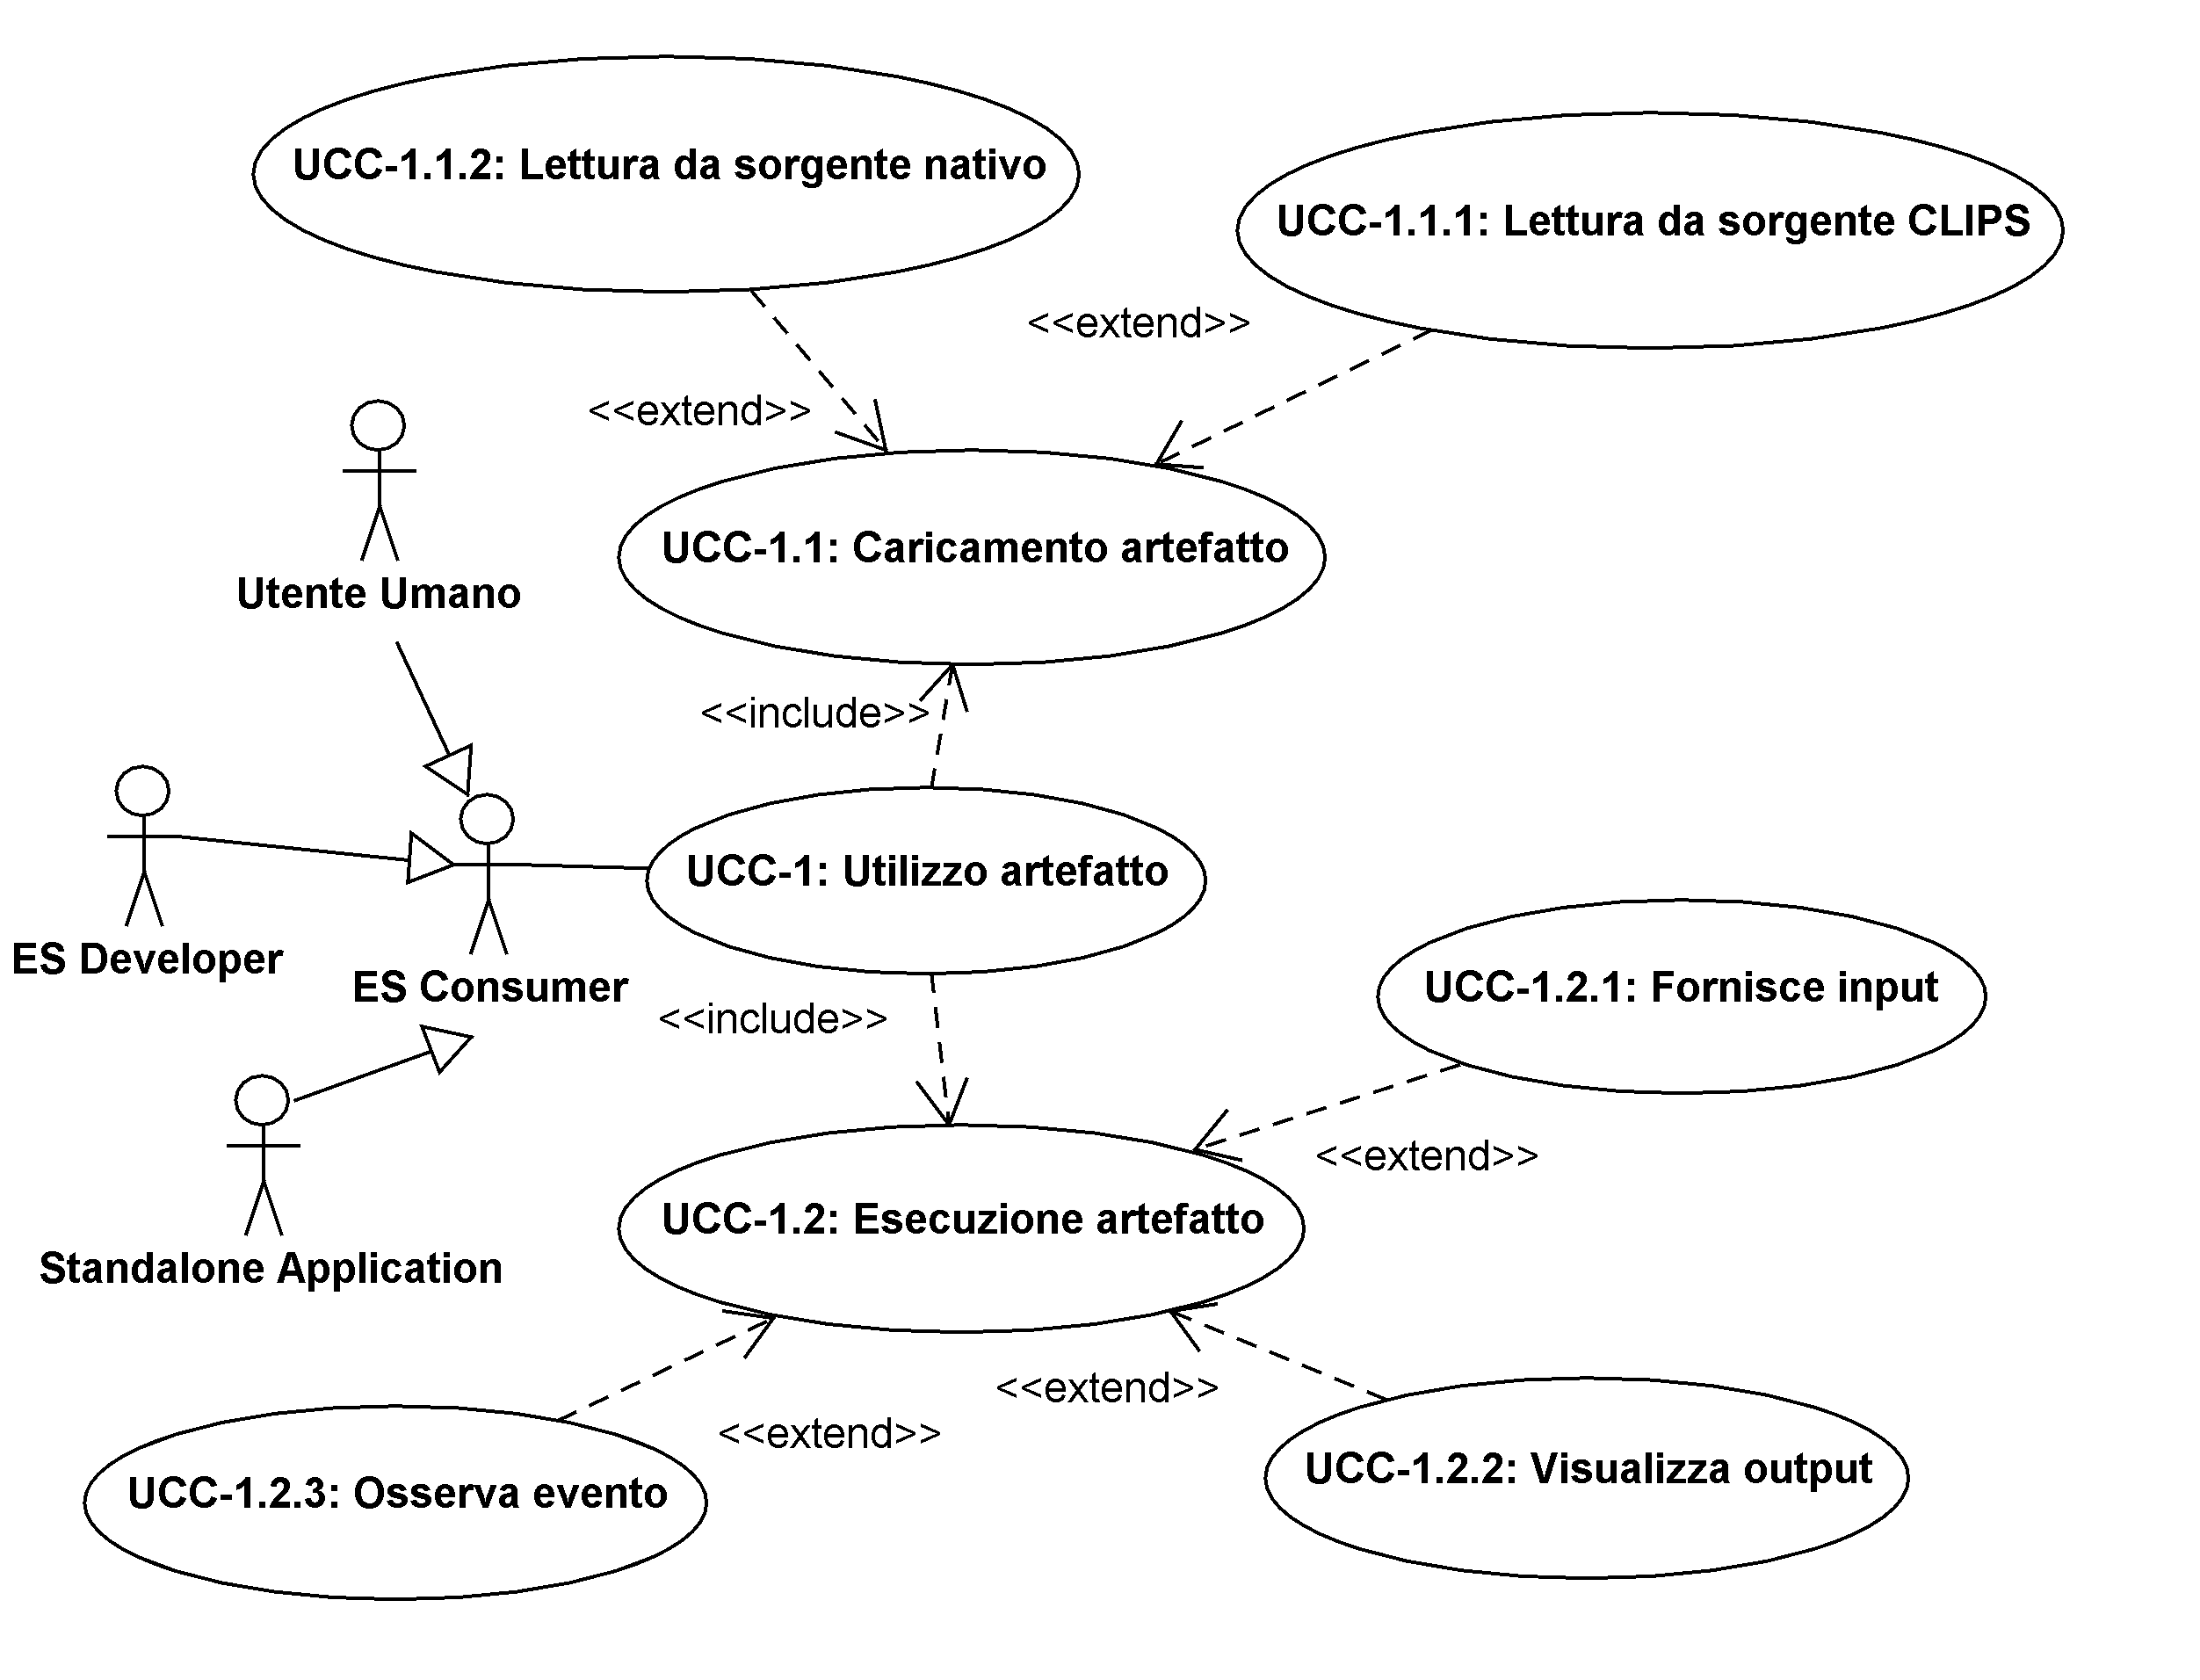
\includegraphics[width=1\textwidth]{Immagini/Capitolo2/UseCases/UCC-1.png}
\caption{Diagramma dei casi d'uso UCC-1}\label{fig:uc-ucc-1}
\end{figure}


\begin{itemize}
	\item \textbf{Attori:} ES Consumer
	\item \textbf{Scopo e descrizione:} un ES Consumer deve poter utilizzare un artefatto precedentemente creato, caricandolo e successivamente eseguendolo.
	\item \textbf{Pre-condizioni:} il software è correttamente configurato nel sistema
	\item \textbf{Post-condizioni:} il software ha eseguito tutte le operazioni desiderate
	\item \textbf{Flusso principale degli eventi:}
		\begin{enumerate}
			\item l'ES Consumer richiede al software di effettuare il caricamento di un artefatto (si veda caso d'uso \emph{UCC-1.1}).
			\item l'ES Consumer richiede al software di eseguire un artefatto (si veda caso d'uso \emph{UCC-1.2}).
		\end{enumerate}
\end{itemize}


\paragraph{UCC-1.1: Caricamento artefatto}

La descrizione comprende quelle dei casi d'uso \emph{UCC-1.1.1} e \emph{UCC-1.1.2} in quanto identici, a meno del formato con il quale l'artefatto viene fornito.

\begin{itemize}
	\item \textbf{Attori:} ES Consumer
	\item \textbf{Scopo e descrizione:} un ES Consumer deve avere la possibilità di caricare nel sistema un artefatto formalizzato in codice sorgente nativo o codice sorgente CLIPS
	\item \textbf{Pre-condizioni:} il software è correttamente configurato nel sistema
	\item \textbf{Post-condizioni:} il software ha eseguito le operazioni di caricamento ed il suo stato rispecchia quello descritto nell'artefatto
	\item \textbf{Flusso principale degli eventi:}
		\begin{enumerate}
			\item l'ES Consumer richiede al software di caricare un artefatto
			\begin{itemize}
				\item l'ES Consumer può fornire un artefatto in formato nativo
				\item l'ES Consumer può fornire un artefatto in formatto CLIPS
			\end{itemize}
			\item Il software analizza l'artefatto
			\item Il software esegue il caricamento dei costrutti contenuti nell'artefatto
		\end{enumerate}
	\item \textbf{Flusso alternativo:}
		\begin{enumerate}
			\setcounter{enumi}{2}
			\item se l'ES Consumer ha fornito un artefatto in formato non valido, il software notifica l'errore fornendo la motivazione e la posizione del problema
		\end{enumerate}
\end{itemize}

\paragraph{UCC-1.2: Esecuzione artefatto}

\begin{itemize}
	\item \textbf{Attori:} ES Consumer
	\item \textbf{Scopo e descrizione:} l'ES Consumer deve poter eseguire un artefatto caricato nel sistema. Se l'interazione lo richiede, l'ES Consumer deve essere in grado di fornire informazioni aggiuntive, osservare l'accadimento di un evento e osservare l'output fornito dal sistema
	\item \textbf{Pre-condizioni:} il software ha correttamente caricato un artefatto ed attende istruzioni.
	\item \textbf{Post-condizioni:} il software ha correttamente eseguito le operazioni previste dall'artefatto.
	\item \textbf{Flusso principale degli eventi:}
		\begin{enumerate}
			\item l'ES Consumer richiede l'esecuzione di un artefatto
			\item il sistema esegue le operazioni previste dall'artefatto (si vedano i casi d'uso \emph{UCC-1.2.1}, \emph{UCC-1.2.3})
			\item il sistema fornisce all'ES Consumer i risultati dell'esecuzione		
		\end{enumerate}
	\item \textbf{Flusso alternativo:} 
		\begin{enumerate}
			\setcounter{enumi}{1}
			\item se un'operazione specificata nell'artefatto genera errori, il sistema notifica l'errore all'ES Consumer fornendo informazioni sulla natura del problema.
			\item il sistema ritorna nello stato iniziale
		\end{enumerate}
\end{itemize}


\subparagraph{UCC-1.2.1: Fornisce input}

\begin{itemize}
	\item \textbf{Attori:} ES Consumer
	\item \textbf{Scopo e descrizione:} l'ES Consumer fornisce informazioni aggiuntive 
	\item \textbf{Pre-condizioni:} il sistema richiede informazioni aggiuntive per completare l'esecuzione di un artefatto
	\item \textbf{Post-condizioni:} il sistema prosegue l'esecuzione
	\item \textbf{Flusso principale degli eventi:}
		\begin{enumerate}
			\item il sistema richiede informazioni aggiuntive
			\item l'ES Consumer fornisce le informazioni nelle forme previste dall'artefatto
			\item il sistema valuta le informazioni fornite
			\item il sistema elabora le informazioni fornite
		\end{enumerate}
	\item \textbf{Flusso alternativo:} 
		\begin{enumerate}
			\setcounter{enumi}{2}
			\item il sistema notifica l'invalidità delle informazioni fornite
			\item lo scenario riprende dal punto 1 del flusso principale
		\end{enumerate}
\end{itemize}


\subparagraph{UCC-1.2.2: Visualizza output}

\begin{itemize}
	\item \textbf{Attori:} ES Consumer
	\item \textbf{Scopo e descrizione:} l'ES Consumer deve essere in grado di valutare l'output fornito dal sistema al termine di un'operazione
	\item \textbf{Pre-condizioni:} il sistema è pronto ad esegue un'operazione
	\item \textbf{Post-condizioni:} il sistema è pronto ad eseguire una nuova operazione
	\item \textbf{Flusso principale degli eventi:}
		\begin{enumerate}
			\item il sistema esegue un'operazione
			\item il sistema fornisce una visualizzazione del risultato
			\item l'ES Consumer valuta il risultato
		\end{enumerate}
\end{itemize}


\subparagraph{UCC-1.2.3: Osserva evento}

\begin{itemize}
	\item \textbf{Attori:} ES Consumer
	\item \textbf{Scopo e descrizione:} l'ES Consumer deve essere in grado di ricevere notifica del verificarsi di un evento
	\item \textbf{Pre-condizioni:} il sistema è pronto ad eseguire un'operazione
	\item \textbf{Post-condizioni:} il sistema è pronto ad eseguire un'operazione
	\item \textbf{Flusso principale degli eventi:}
		\begin{enumerate}
			\item l'ES Consumer richiede al sistema di eseguire un'operazione
			\item il sistema esegue un'operazione
			\item il sistema notifica all'ES Consumer il verificarsi di un evento
			\item l'ES Consumer valuta l'evento
		\end{enumerate}
\end{itemize}